\documentclass[usenames,dvipsnames,8pt,aspectratio=169]{beamer}
\usepackage{amsmath,amsfonts,amssymb}
\usepackage{mathtools}
\usepackage{etex} %for Windows
\usepackage[utf8]{inputenc}
\usepackage[english, russian]{babel} 
%\usepackage{microtype}			% Better interword spacing and additional kerning.
\usepackage{ellipsis}			% Adjusted space with \dots between two words.
\usepackage{graphicx}
\usepackage{pstricks}

\usepackage{xcolor}


\usepackage{changepage}

\usepackage{algorithm}
\usepackage{algpseudocode}
%\usepackage[]{algorithm2e}
%\usepackage{algorithmic}

%\usepackage{tcolorbox}


\usepackage{caption}
\usepackage{subcaption}
%\usepackage{stackengine}


\usepackage{tikz}
\usetikzlibrary{tikzmark,calc}
\usetikzlibrary{positioning, backgrounds}
\usetikzlibrary{arrows, chains, matrix, scopes, patterns, shapes, fit}
\usetikzlibrary{mindmap,trees,shadows}
\usetikzlibrary{decorations.pathreplacing}
%\usetikzlibrary{crypto.symbols}

\usepackage{pgfplots}

\pgfmathdeclarefunction{gauss}{2}{%
	\pgfmathparse{1/(#2*sqrt(2*pi))*exp(-((x-#1)^2)/(2*#2^2))}%
}


\tikzset{
	invisible/.style={opacity=0},
	visible on/.style={alt={#1{}{invisible}}},
	alt/.code args={<#1>#2#3}{%
		\alt<#1>{\pgfkeysalso{#2}}{\pgfkeysalso{#3}} % \pgfkeysalso doesn't change the path
	},
}

\newcommand\strikeout[2][]{%
	\begin{tabular}[b]{@{}c@{}} 
		\makebox(0,0)[cb]{{#1}} \\[-0.2\normalbaselineskip]
		\rlap{\color{Orange}\rule[0.5ex]{\widthof{#2}}{1.5pt}}#2
\end{tabular}}

\newcommand\Fontvi{\fontsize{11}{13.2}\selectfont}

\usepackage{listings} % for C++ code

\usepackage{braket}
%\usepackage[braket, qm]{qcircuit}



\usepackage[T1]{fontenc}
%\usepackage[sfdefault,scaled=.85]{FiraSans}
%\usepackage{newtxsf}
%\usepackage[nomap]{FiraMono}


\usepackage{changepage}



\usefonttheme[onlymath]{serif}
\renewcommand\sfdefault{cmbr}

\renewcommand{\bfdefault}{sb}

\definecolor{CharCoalDark}{RGB}{13, 16, 19}
\definecolor{Orange}{RGB}{255, 165,0}
\definecolor{DarkOrange}{RGB}{255, 165,0}
\definecolor{LightSalmon}{RGB}{255, 160, 122}
\definecolor{MapleWood}{RGB}{241, 195, 142}
\definecolor{Redwood}{RGB}{210, 173, 169}
\definecolor{LeafGreen}{RGB}{34, 139,  34}
\definecolor{Coral}{RGB}{255, 127, 80}
\definecolor{DarkTurquoise}{RGB}{0, 206, 209}

%\newtheorem{defRus}{Определение}
%\newtheorem{thmRus}{Теорема}
%s\newtheorem{corRus}{Следствие}


\setbeamercolor{background canvas}{bg=CharCoalDark}

\setbeamerfont{title}{series=\bfseries}
\setbeamercolor{title}{fg=Orange}
\setbeamercolor{section in toc}{fg=white}
\setbeamercolor{frametitle}{fg=Orange}
\setbeamercolor{normal text}{fg=white}
%\setbeamercolor{normal text}{fontsize=12pt}
\setbeamercolor{itemize item}{fg=Orange}
\setbeamercolor{enumerate item}{fg=Orange}
\setbeamercolor{enumerate item item}{fg=Orange}
\setbeamercolor{itemize item item}{fg=Orange}
\setbeamercolor{enumerate item}{fg=Orange}
\setbeamercolor{block title}{bg=DarkOrange,fg=white}
\setbeamerfont{block title}{series=\bfseries}

\setbeamertemplate{itemize item}[circle]
\setbeamertemplate{eumerate subitem}{\color{Orange}[$\checkmark$]}
\setbeamertemplate{itemize subitem}{\color{Orange}\Large$\textbullet$}
\setbeamertemplate{itemize subitem}{\color{Orange} \tiny $\blacksquare$}

% footnote without a marker
\newcommand\blfootnote[1]{%
	\begingroup
	\renewcommand\footnoterule{}
	\renewcommand\thefootnote{}\footnote{#1}%
	\addtocounter{footnote}{-1}%
	\endgroup
}


\usepackage[absolute,overlay]{textpos} %to clip to a corner
\newcommand\FrameText[1]{%
	\begin{textblock*}{\paperwidth}(\textwidth-35pt, 10 pt)
		\raggedright #1\hspace{.5em}
\end{textblock*}}

\makeatletter
\let\save@measuring@true\measuring@true
\def\measuring@true{%
	\save@measuring@true
	\def\beamer@sortzero##1{\beamer@ifnextcharospec{\beamer@sortzeroread{##1}}{}}%
	\def\beamer@sortzeroread##1<##2>{}%
	\def\beamer@finalnospec{}%
}
\makeatother

\AtBeginSection[]
{
	\begin{frame}<beamer>
		\frametitle{Outline}
		\tableofcontents[currentsection]
	\end{frame}
}


\title{Лекция №10 \\[10pt]
	Часть 1. Криптографические протоколы. TLS}

\date{ Елена Киршанова \\  \textbf{Курс ``Основы криптографии''} \\  }



\setbeamertemplate{navigation symbols}{} %removes navigation

% proper highlightling of a code-snippet
\lstset{language=C++,
	keywordstyle=\color{magenta},
	stringstyle=\color{Goldenrod},
	commentstyle=\color{gray},
	breaklines=false,
	%morecomment=[l][\color{magenta}]{\#}
}


% ==================================================================
% Definitions for this paper
% ==================================================================
\mathchardef\hyphen="2D

\usepackage{multirow}
\usepackage{multicol} % For multiple coloumn environments
%\usepackage{stmaryrd} % For set brackets
% \setlength{\columnsep}{15pt} % Defining the coloumn seperation
% \setlength{\columnseprule}{1pt} % Place a line between coloumns
% \newcommand{\tab}{\hspace*{2em}}

%subscripts

\newcommand*\SmallTextScript[2]{{\mathchoice{\displaystyle #2}
		{\textstyle #2}%dito
		{\scalebox{#1}{\ensuremath{\scriptstyle #2}}}%
		{\scalebox{#1}{\ensuremath{\scriptscriptstyle #2}}}%
}}


% ADVERSARIES AND SUCH
\newcommand*{\poly}{\ensuremath{\mathrm{poly}}}
\newcommand*{\eps}{\ensuremath{\varepsilon}}
\newcommand*{\alg}{\ensuremath{\mathcal{A}}}

% GROUPS/DISTRIBUTIONS/SETS/LISTS
\newcommand{\N}{{{\mathbb N}}}
\newcommand{\Z}{{{\mathbb Z}}}
\newcommand*{\IZ}{\ensuremath{\mathbb{Z}}}
\newcommand*{\IN}{\ensuremath{\mathbb{N}}}
\newcommand*{\IQ}{\ensuremath{\mathbb{Q}}}
\newcommand{\R}{{{\mathbb R}}}
\newcommand*{\IR}{{{\mathbb R}}}
\newcommand{\Zp}{\ints_p} % Integers modulo p
\newcommand{\Zq}{\ints_q} % Integers modulo q
\newcommand{\Zn}{\ints_N} % Integers modulo N
\newcommand{\F}{\ensuremath{\mathbb{F}}}
\newcommand{\CC}{\ensuremath{\mathbb{C}}}

\newcommand{\GF}{\ensuremath{\mathbb{F}_2}}
\newcommand{\GFn}{\ensuremath{\mathbb{F}^n_2}}

%%% ALGORITHMS/PROCEDURES %%%
\newcommand{\Dec}{\textsf{Dec}}
\newcommand{\Enc}{\textsf{Enc}}
\newcommand{\KeyGen}{\textsf{KeyGen}}
\newcommand{\Gen}{\textsf{Gen}}
\newcommand{\sk}{\textsf{sk}}
\newcommand{\pk}{\textsf{pk}}
\newcommand{\vk}{\textsf{vk}}
\newcommand{\mesS}{\ensuremath{\mathcal{M}}}
\newcommand{\keyS}{\ensuremath{\mathcal{K}}}
\newcommand{\cipS}{\ensuremath{\mathcal{C}}}
\newcommand{\tagS}{\ensuremath{\mathcal{T}}}
\newcommand{\mactag}{\textsf{tag}}
\newcommand{\Hash}{\ensuremath{\mathcal{H}}}
\newcommand{\EID}{\ensuremath{\mathtt{EphID}}}


\newcommand{\adv}{\ensuremath{\mathcal{A}}}

\newcommand{\LWE}{\mathsf{LWE}}
\newcommand{\DCP}{\mathsf{DCP}}
\newcommand{\EDCP}{\mathsf{EDCP}}
\newcommand{\UEDCP}{\mathsf{U \text{-} EDCP}}
\newcommand{\GEDCP}{\mathsf{G \text{-} EDCP}}



%% Landau and proba
\newcommand{\bigO}{\mathcal{O}}
\newcommand*{\OLandau}{\bigO}
\newcommand*{\WLandau}{\Omega}
\newcommand*{\xOLandau}{\widetilde{\OLandau}}
\newcommand*{\xWLandau}{\widetilde{\WLandau}}
\newcommand*{\TLandau}{\Theta}
\newcommand*{\xTLandau}{\widetilde{\TLandau}}
\newcommand{\smallo}{o} %technically, an omicron
\newcommand{\wLandau}{\omega}
\newcommand{\negl}{\mathrm{negl}}
\newcommand*\PROB\Pr 
\DeclareMathOperator*{\EXPECT}{\mathbb{E}}
\DeclareMathOperator*{\VARIANCE}{\mathbb{V}}
\DeclareMathOperator*{\LOGBIAS}{\mathbb{LB}}

\newcommand{\supp}{\ensuremath{\mathsf{sup}}}
\newcommand{\Distr}{\ensuremath{\mathcal{D}}}

% Lattices

% \newcommand{\coset}{\Lambda} % Lambda Lattice
% \newcommand{\cosetPerp}{\Lambda^{\bot}} % Lambda_Perp Lattice
% \newcommand{\gadget}{\textbf{G}} %Gaget matrix
% \newcommand{\mes}{\textbf{m}} %message vector
% \newcommand{\AMat}{\textbf{A}} %A matrices
% \newcommand{\BMat}{\textbf{B}} %B matrices
% \newcommand{\RMat}{\textbf{R}} %R matrices
% \newcommand{\HMat}{\textbf{H}} %H matrices
% \newcommand{\XMat}{\textbf{X}} %H matrices
% \newcommand{\mbar}{\bar{m}} %mBar dimension
% % \newcommand{\gauss}{\mathcal{D}} % gaussian distribution
% \newcommand{\Id}{\textbf{I}} % Identity matrix
% \newcommand{\er}{\textbf{e}} % gaussian distr. vectors
% % \newcommand{\cipher}{\textit{c}} % ciphertext
% \newcommand{\Olwe}{\mathcal{O}_{\textsf{LWE}}} %LWE oracle
% \newcommand{\OSample}{\mathcal{O}_{Sample}} %LWE oracle
% \newcommand{\SigmaB}{\boldsymbol{\Sigma}} %semi-deifinite matrix Sigma%
% % \newcommand{\mods}{\text{ mod}}


%Vectors and Matrices

\newcommand{\AMat}{\mathbf{A}} %A matrices
\newcommand{\BMat}{\mathbf{B}} %B matrices
\newcommand{\DMat}{\mathbf{D}} %Diagonal


\newcommand{\HMat}{\ensuremath{\mathbf{H}}}
\newcommand{\QMat}{\ensuremath{\mathbf{Q}}}
\newcommand{\Id}{\ensuremath{\mathbf{I}}}
\newcommand{\ZeroM}{\textbf{0}} % Zero matrix

\newcommand{\avec}{\ensuremath{\mathbf{a}}}
\newcommand{\bvec}{\ensuremath{\mathbf{b}}}
\newcommand{\cvec}{\ensuremath{\mathbf{c}}}
\newcommand{\evec}{\ensuremath{\mathbf{e}}}
\newcommand{\rvec}{\ensuremath{\mathbf{r}}}
\newcommand{\svec}{\ensuremath{\mathbf{s}}}
\newcommand{\tvec}{\ensuremath{\mathbf{t}}}
\newcommand{\vvec}{\ensuremath{\mathbf{v}}}
\newcommand{\zvec}{\ensuremath{\mathbf{z}}}
\newcommand{\xvec}{\ensuremath{\mathbf{x}}}
\newcommand{\yvec}{\ensuremath{\mathbf{y}}}
\newcommand{\uvec}{\ensuremath{\mathbf{u}}}
\newcommand{\zerovec}{\ensuremath{\mathbf{0}}}

\newcommand{\nth}{^{\mathrm{th}}}
\newcommand{\nd}{^{\mathrm{nd}}}

\newcommand{\RepMMT}{\ensuremath{\mathcal{R}_{\protect\SmallTextScript{0.70}{\texttt{MMT}}}}}
\newcommand{\RepBJMM}{\ensuremath{\mathcal{R}_{\protect\SmallTextScript{0.70}{\texttt{BJMM}}}}}
\newcommand{\XOR}{\ensuremath{\mathtt{3XOR}}}


% % % % % \newcommand{\mb}[1]{\mathbf{#1}} % does not compile otherwise
%%% Removed by Gotti; this is just asking to screw up with packages that (properly) define \mb (mathbold)

% \newcommand{\bL}{\|\bvec_1\|} % b1 length that appears way too often
% \newcommand{\dL}{\|\dvec_1\|} % b1 length that appears way too oftend

%Norms and Scalar products

\newcommand*\abs[1]{\left\lvert#1\right\rvert}
\newcommand*\norm[1]{\left\lVert#1\right\rVert}
\newcommand*\normalabs[1]{\lvert#1\rvert} 
\newcommand*\normalnorm[1]{\lVert#1\rVert}
\newcommand*\bignorm[1]{\bigl\lVert#1\bigr\rVert}
\newcommand*\bigabs[1]{\bigl\lvert#1\bigr\rvert}
\newcommand*\Bigabs[1]{\Bigl\lvert#1\Bigr\rvert}
\newcommand*{\ScProd}[2]{\ensuremath{\langle#1\mathbin{,}#2\rangle}} %Scalar Product
% \newcommand*{\ScProd}[2]{\ensuremath{\langle#1 \:{,}\:#2\rangle}} %Scalar Product
\newcommand*{\bigScProd}[2]{\ensuremath{\bigl\langle#1\mathbin{,}#2\bigr\rangle}} %Scalar Product
\newcommand*{\BigScProd}[2]{\ensuremath{\Bigl\langle#1\mathbin{,}#2\Bigr\rangle}} %Scalar Product
\newcommand{\dist}{\ensuremath{\text{dist}}}


%Some other math operators

\DeclareMathOperator{\Span}{Span} %span of vectors
\DeclareMathOperator{\vol}{\mathrm{vol}} %volume
\DeclareMathOperator{\LW}{LambertW} %Lambert W function
\DeclareMathOperator{\SD}{SD}
\DeclareMathOperator{\gradient}{grad}
\DeclareMathOperator{\TRACE}{Tr}
\newcommand*{\dDR}{\mathrm{d}} %de-Rham-Differential (the d in dx, dy, dz and so on)


%Lists
\renewcommand{\L}{\ensuremath{\mathcal{L}}}

\renewcommand{\P}{\ensuremath{\mathcal{P}}}

\newcommand*{\Lout}{\ensuremath{\L_{\mkern-0.5mu\protect\SmallTextScript{0.85}{\textup{out}}}}}
\newcommand*{\Sout}{\ensuremath{S_{\mkern-0.5mu\protect\SmallTextScript{0.85}{\textup{out}}}}}
\newcommand{\wt}{\ensuremath{\mathit{wt}}}


\newcommand*{\softO}{\widetilde{\bigO}}

\newcommand{\const}{\mathsf{c}} 


\newcommand{\transpose}{\mkern0.7mu^{\mathsf{ t}}}

%proper overline reduced by 1.5mu
\newcommand{\overbar}[1]{\mkern 1.5mu\overline{\mkern-1.5mu#1\mkern-1.5mu}\mkern 1.5mu}

\DeclareMathOperator{\erf}{erf} %error function
\DeclareMathOperator{\erfc}{erfc} %complementary error function
\newcommand{\Er}{\ensuremath{\mathrm{Er}}} %complementary error function


% LATTICES

\newcommand{\Lat}{\ensuremath{\mathcal{L}}}
\newcommand*{\Sphere}[1]{\ensuremath{\mathsf{S}^{#1}}}
%\DeclareMathOperator{\Conf}{Conf}
\newcommand{\Conf}{\mathcal{C}}

%Thick line for table
\setlength{\doublerulesep}{0pt}
\newcommand{\thickline}{\hline\hline\hline}


%circled text
\newcommand*\circled[1]{\tikz[baseline=(char.base)]{
    \node[shape=circle,draw,inner sep=0.3 pt] (char) {\scriptsize #1};}}


%Fix Algorithmicx package
\def\NoNumber#1{{\def\alglinenumber##1{}\State #1}\addtocounter{ALG@line}{-1}}

%For comments
\newcommand{\GColor}{ForestGreen}  %Damiens' color
\newcommand{\EColor}{MidnightBlue} %Elena's color

\newcommand*{\E}[1]{{\color{\EColor} #1} } 
\newcommand*{\G}[1]{{\color{\GColor} #1} } 

%Proper limit with the subscript underneath
% \newcommand{\Lim}[1]{\raisebox{0.5ex}{\scalebox{0.8}{$\displaystyle \lim_{#1}\;$}}}


%TIKZ dense dotted pattern

\pgfdeclarepatternformonly{my dots}{\pgfqpoint{-1pt}{-1pt}}{\pgfqpoint{2.0pt}{2.0pt}}{\pgfqpoint{2pt}{2pt}}%
{
	\pgfpathcircle{\pgfqpoint{0pt}{0pt}}{.35pt}
	\pgfpathcircle{\pgfqpoint{1pt}{1pt}}{.35pt}
	\pgfusepath{fill}
}


\tikzset{
	master/.style={
		execute at end picture={
			\coordinate (lower right) at (current bounding box.south east);
			\coordinate (upper left) at (current bounding box.north west);
		}
	},
	slave/.style={
		execute at end picture={
			\pgfresetboundingbox
			\path  (lower right)rectangle (upper left) ;
		}
	}
} %all defs
\begin{document}
	
\begin{frame}
	\titlepage
\end{frame}

\begin{frame}{We've looked at}
\LARGE
\centering
	Гибрид \\[10pt]
	{ \color{Orange} Обмен ключами /KEM, безопасные против активных атакующий + AEAD --}  \\[10pt]
	центральный в современных протоколах.

\end{frame}



\begin{frame}{TLS: Transport Layer Security(Протокол защиты транспортного уровня)}

\Large
%\begin{center}
{\color{Orange}TLS -- } протокол установления и поддержки безопасного соединения между клиентов и серверов по Интернету. 
%\end{center}
\vspace{10pt}
\begin{columns}
	\begin{column}{0.6\textwidth}
		I. SSL = Secure Socket Layer   \\[10pt]
		\begin{itemize}
			{\large
			\item SSLv1 (1994) — не опубликован 
			\item SSLv2 (1995) — взлома
			\item SSLv3 (1996) — поддерживается
			}
		\end{itemize}
	\vspace{10pt}
	II. TLS = Transport Layer Security  \\[10pt]
	\begin{itemize}
		{\large
		\item TLS 1.0 (1999) — RFC 2246
		\item TLS 1.1 (2006) — RFC 4346
		\item TLS 1.2 (2008) — RFC 5246
		\item TLS 1.3 (2018) — RFC 8448 \\
		\url{https://datatracker.ietf.org/doc/rfc8446/}
		
	}
	\end{itemize}
	\end{column}

	\begin{column}{0.35\textwidth}
	
		\vspace{75pt}
		
		{
			\huge
			{\color{Orange} Стандарты IETF }
		}
	\end{column}
\end{columns}

\vfill
\small
RFC = Request for Comments\\
IETF = Internet Engineering Task Force

\end{frame}


\begin{frame}{Структура протокола TLS}
	\LARGE
	\begin{center}
		\begin{tabular}{c c c }
			{\color{Orange}\texttt{Клиент}}&  {\color{Orange}{Фаза 1} Handshake}   & 	{\color{Orange}\texttt{Сервер} } \\
			& {\Large выбор примитивов, параметров}  & \\ 
			& {\Large аутентификация (как мин. сервера) }  & \\ 
			& {\Large генерация общего ключа}  &  \\[10pt]
			& {\Huge $\downarrow k$}& \\ [10pt]
			&  {\color{Orange}{Фаза  2} TLS record protocol}   &  \\
			& {\Large шифрование данных с помощью AEAD с ключом  $k$}  & \\ 
		\end{tabular}
	\end{center}

\vspace{10pt}
TLS живёт на транспортном уровне TCP/IP, т.e., пакеты приходят в корректном порядке.
\end{frame}


\begin{frame}{Где живёт TLS}
\centering
\begin{tikzpicture}
	\draw [draw=white] (-5.,11) rectangle (5,12.0) node[pos=0.5] {\LARGE HTTPS (Application)};
	
	\draw[-stealth, thick] (-3, 10.8) -- (-3, 9.8);
	\draw[-stealth, thick] (0, 10.8) -- (0, 9.8);
	\draw[-stealth, thick] (3, 10.8) -- (3, 9.8);
	
	\draw [draw=white] (-5.,7.5) rectangle (5,9.5);
	\node[rotate=90, color=white] at (-4.5, 8.3) {\LARGE TLS};
	\draw [draw=white] (-4.,8.5) rectangle (-2, 9.4) node[pos=0.5] {\Large Handshake};
	\draw [draw=white] (-1.8,8.5) rectangle (0.7, 9.4) node[pos=0.5] {\Large Encryption ON};
	\draw [draw=white] (0.9,8.5) rectangle (2.7, 9.4) node[pos=0.5] {\Large Alert};
	\draw [draw=white] (3.0,8.5) rectangle (4.9, 9.4) node[pos=0.5, align=left] {\small App. data \\ protocol};
	\draw [draw=white] (-4,7.7) rectangle (4.9,8.2) node[pos=0.5] {\Large Record protocol};
	
	\draw[-stealth, thick] (-3, 7.2) -- (-3, 6.2);
	\draw[-stealth, thick] (0, 7.2) -- (0, 6.2);
	\draw[-stealth, thick] (3, 7.2) -- (3, 6.2);
	
	
	\draw [draw=white] (-5.,4.5) rectangle (5,5.5) node[pos=0.5] {\LARGE TCP};
\end{tikzpicture}
\vfill Слайд взят из презентации K.Patterson \url{https://www.isg.rhul.ac.uk/~kp/TLSwheredowestand.pdf}
	
\end{frame}



\begin{frame}{Фаза1: TLS Handshake}
\begin{adjustwidth}{-2.0em}{-1.5em}
\begin{center}
	\begin{tabular}{l l l }
		{\Large \color{Orange}\texttt{Клиент}}&    & \hspace{20pt} {\Large {\color{Orange}\texttt{Сервер}}}  \\
		&
		\begin{tikzpicture}[remember picture, overlay]
			\draw[-stealth, thick] (-0.5,0) -- (3.5, 0) node[above,midway] { $\pk_c = g^{a}$, Nonce $N_c$, offer };
		\end{tikzpicture} &  \\
		&{\small offer: список шифров клиентов} & \pause {1. Выбор шифра}  \\
		&& {\small (Enc. scheme, hash) }  \\
		&& {\small 2. Вычисляет {\color{Orange}$k_{\text{shared}} = g^{ab}$}}\\
		&& {\small $k_{\text{sh}}$ -- ключ шифрования сервера }\\
		&& {\small $k_{\text{sm}}$-- ключа MAC'a сервера  }  \\
		&\begin{tikzpicture}[remember picture, overlay]
		\draw[stealth-, thick] (-0.5,0) -- (3.5, 0) node[above,midway] { $\pk_s = g^{b}$, Nonce $N_s$, режим };
		\end{tikzpicture} & {\small $k_{\text{ch}}$ - ключ шифрования клиента }\\
		&{\small mode: chosen cipher suits}  & {\small $k_{\text{cm}}$ -ключа MAC'a  клиента } \pause \\
	3. Вычисляет {\color{Orange}$k_{\text{shared}} = g^{ab}$}	&& \\
	{ $k_{\text{sh}},k_{\text{sm}},k_{\text{ch}},k_{\text{cm}}$} && \pause \\
	&
	\begin{tikzpicture}[remember picture, overlay]
	\draw[stealth-, thick] (-0.5,0) -- (3.5, 0);
	\end{tikzpicture} &\\[-2pt]
	& \small $ c_1 = \Enc(k_{\text{sh}}, \text{ Cert. request})$ & \\
	&\small $c_2 = \Enc(k_{\text{sh}}, \text{ Cert. Server})$ & \\
	&\small $c_3 = \Enc(k_{\text{sh}}, \Sign(\text{transcript}))$ & \\
	&\small $c_4 = \Enc(k_{\text{sh}}, \MAC(k_{\text{sm}}, \text{transcript}))$ & \pause \\
	&
	\begin{tikzpicture}[remember picture, overlay]
	\draw[-stealth, thick] (-0.5,0) -- (3.5, 0);
	\end{tikzpicture} &\\[-2pt]
	&\small $c_5 = \Enc(k_{\text{ch}}, \text{ Cert. Client})$ &  \\
{\large \color{Orange}$(k_{c\rightarrow s},k_{s\rightarrow c}) = \Hash(\text{\small transcript})$}	&\small $c_6 = \Enc(k_{\text{ch}}, \Sign(\text{transcript}))$ & {\large \color{Orange}$(k_{c\rightarrow s},k_{s\rightarrow c}) = \Hash(\text{\small transcript})$}\\
	&\small $c_7 = \Enc(k_{\text{ch}}, \MAC(k_{\text{cm}}, \text{transcript}))$ & \\
	\end{tabular}
\end{center}


\end{adjustwidth}

\end{frame}

\begin{frame}{Фаза2: TLS Record Layer}
	\Large Данные = $\left[m_1, \ldots, m_s\right]$
	\begin{center}
		\begin{tabular}{c c c }
			{\Large \color{Orange}\texttt{Клиент}}&   & {\Large {\color{Orange}\texttt{Сервер}}} \\
			$k_{c\rightarrow s}$&  & $k_{c\rightarrow s}$\\ 
			$k_{s\rightarrow c}$&  & $k_{s\rightarrow c}$  \\ 
			& {\large$\underbrace{
					\left[
					\texttt{Meta data} || \;
					m_i \; || \;
					\texttt{Nonce}
					\right]}$}  &   \\ 
			&$\xrightarrow{ \hspace{1.0em}  \Large \text{ \hspace{30pt} AES-GCM-AEAD}(k_{c\rightarrow s}) \hspace{3.4em} }$   &  \\
		\end{tabular}
	\end{center}
\end{frame}

\begin{frame}{Безопасность}
	\Large
	\begin{itemize}
		\itemsep 8pt
		\item {\color{Orange} Протокол Alert } ответственен за обработку ошибок, предупреждений и окончания сессий  
		\item Существуют формальные доказательства безопасности  TLS 1.3 
		\item {\color{Orange} Обновление ключа:} получив сообщение \texttt{KeyUpdate} Клиент и Сервера обновляют $k_{c\rightarrow s}, k_{s\rightarrow c}$
		\item {\color{Orange}{Возобновление сессии (Pre-shared key handshake)}}: более эффективная фаза Handshake Phase, если между клиентов и сервером ранее уже были установлены сессии
		\item {\color{Orange}Forward secrecy:} если злоумышленник получает общий ключ, \emph{предыдущие} сообщения остаются конфиденциальными.
	\end{itemize}
\end{frame}


\begin{frame}{Наборы алгоритмов в TLS 1.3}
\Large
		\begin{tabular}{l l l l }
		\hspace{-20pt}	\textbf{\color{Orange}{Обмен ключами}} & \textbf{\color{Orange}{Сертификаты}} & \textbf{\color{Orange}{Сим. шифрование }} & \textbf{\color{Orange}{Хэш-функции}} \\[10pt]
		\hspace{-20pt}	ECDHE & ECDSA & AES\_256\_GCM & (H)SHA\_384 \\[5pt]
		\hspace{-20pt}	DHE & RSA & CHACHA20\_Poly1350 & (H)SHA\_256 \\[5pt]
		\hspace{-20pt}	{\color{gray}RSA} &  & AES\_128\_GCM & (H)SHA1 \\[15pt]
		\hspace{-20pt}	 &  & AES\_256\_CBC &  \\[5pt]
		\hspace{-20pt}	 &  & AES\_128\_CBC &  \\[15pt]
		\hspace{-20pt}	 &  & {\color{gray}3DES\_CBC} &  \\[10pt]
		\end{tabular}
\end{frame}

\begin{frame}{Декодирование названия шифра}
	\begin{center}
		\LARGE {\color{Orange} TLS 1.2} \\[60pt]
		
		
		{\color{Orange}TLS}\_{\color{LightSalmon}ECDHE}\_{\color{Coral}RSA}\_WITH\_{\color{MapleWood}AES\_128\_GCM}\_{\color{Redwood}SHA256}
		
	\begin{tikzpicture}[remember picture, overlay,
	every node/.append style = { align = center, minimum height = 10pt,}
	 ]
	\draw[-stealth, thick] (-4.5,1) -- (-4.5, 2) node[above] {\color{Orange} название протокола};
	\draw[-stealth, thick] (-3.2,0.3) -- (-3.2, -0.5) node[below] {\color{LightSalmon} обмен ключами};
	\draw[-stealth, thick] (-1.7,1) -- (-1.7, 2) node[above] {\color{Coral} аутентификация};
	\draw[-stealth, thick] (1.5, 0.3) -- (1.5, -0.5) node[below] {\color{MapleWood} сим.\  шифрование};
	\draw[-stealth, thick] (4.2,1) -- (4.2, 2) node[above] {\color{Redwood} MAC};
	\end{tikzpicture} 

	\end{center}

	\vspace{30pt}
	\begin{center}
		\LARGE {\color{Orange} TLS 1.3 наборы шифров по умолчанию:}\\
	\end{center}
\Large
		TLS\_AES\_256\_GCM\_SHA384 \\[5pt]
		TLS\_CHACHA20\_POLY1305\_SHA256 \\[5pt]
		TLS\_AES\_128\_GCM\_SHA256 \\[5pt]
	
\end{frame}

\begin{frame}{Данные Вашего браузера / сервера }
	\Large
	\centering
	Используйте \\[5pt]
	\url{https://www.ssllabs.com/index.html} \\[5pt]
	для получения поддерживаемых версий SSL/TLS Вашего браузера или сервера\\[15pt]
	
\end{frame}

%\begin{frame}
%Part II \\ [10pt]
%
%\color{Orange}
%\Huge Secure Messaging
%
%\end{frame}
%
%\begin{frame}{Secure Messaging}
%	\Large
%	A {\color{Orange} Secure Messaging} (SM) allow two parties to communicate with each other with the following security conditions being satisfied:
%	\large
%	\pause
%	\begin{itemize}
%		\itemsep5pt
%		\item {\color{Orange}Correctness}
%		\item {\color{Orange} Privacy:} attacker obtains no information about the messages sent unless a party is compromised
%		\item {\color{Orange} Authenticity:} the attacker cannot change, duplicate or inject messages
%		\item  {\color{Orange} Immediate  decryption}
%		\item {\color{Orange}  Message-loss resilience:} if a message is lost, communication continues
%		\item {\color{Orange} Forward secrecy:} all messages exchanged \emph{before} a compromise remain hidden to an attacker
%		\item {\color{Orange} Post-compromise security: } the parties can recover \emph{after} a compromise
%	\end{itemize}
%	\centering
%\end{frame}
%
%\begin{frame}{Secure Messaging protocol: Signal}
%	\Large
%	{\color{Orange} The Signal Protocol}, designed by Open Whisper Systems, is an example of Secure Messaging.
%	\vspace{20pt}
%	\large
%	\begin{itemize}
%		\itemsep 7pt
%		\item deployed in many apps like WhatsApp, Facebook Messenger, Skype
%		\item every message is encrypted and authenticated using a fresh symmetric key
%		\item satisfies the above security conditions
%	\end{itemize}
%	\vspace{30pt}
%\small 
%Description of Signal: \url{https://signal.org/docs/specifications/doubleratchet/doubleratchet.pdf} \\[5pt]
%It's analysis: \url{https://eprint.iacr.org/2018/1037.pdf} 
%\end{frame}
%
%\begin{frame}{Primitives for SM Protocols}
%\Large
%\[
%	\left.
%	\begin{array}{rrr}
%		\text{Correctness}\\
%		\text{Privacy}\\
%		\text{Authenticity}\\
%		\text{Immediate decryption} \\
%		\text{Message-loss resilience}\\
%		\text{Forward security}
%	\end{array}
%	\right\}\text{AEAD (symmetric primitive)}
%	\]
%AEAD -- Authenticated Encryption with Associated Data \\[20pt]
%\[
%\left.
%\begin{array}{rrr}
%\text{Post-compromise security}
%\end{array}
%\right\}\text{CKA (asymmetric primitive)}
%\]
%CKA -- Continuous Key Agreement
%\end{frame}
%
%\begin{frame}{Signal: high level symmetric part}
%	\begin{center}
%		\begin{tabular}{c c c }
%			{\LARGE \color{Orange}\texttt{A}}&    & {\LARGE \color{Orange}\texttt{B}}  \\
%			{\color{Orange}\texttt{Sender}}&   $\leftarrow k_{\text{shared}} \rightarrow $   & {\color{Orange}\texttt{Receiver}}  \pause \\[10pt]
%			$s_{\text{A},0} \leftarrow \mathtt{InitSender}(k)$& & $s_{\text{B},0} \leftarrow \mathtt{InitReceiver}(k)$ \pause\\[10pt]
%			$s_{\text{A},1}, c_1 \leftarrow \mathtt{Send}(m_1)$& $\xrightarrow{\hspace{5pt}c_1\hspace{5pt}}$ & \\
%			$s_{\text{A},2}, c_2 \leftarrow \mathtt{Send}(m_2)$& $\xrightarrow{\hspace{5pt}c_2\hspace{5pt}}$ & \\
%			& & $s_{\text{B},1}, m_1 \leftarrow \mathtt{Receive}(c_1)$ \\
%			& & $s_{\text{B},2}, m_2 \leftarrow \mathtt{Receive}(c_2)$ \\
%			& $\vdots $& \\
%		\end{tabular}
%	\end{center}
%\pause 
%\begin{itemize}
%	\item think about $\mathtt{Send}$ as of encryption, $\mathtt{Receive}$ as of decryption
%	\item $s_{\text{A},i}$ -- A's $i-\th$ state
%	\item $s_{\text{B},i}$ -- B's $i-\th$ state
%	\item the states should remain secure
%	\item ciphertexts $c_i$ may not come to \texttt{B} in order!
%\end{itemize}
%
%\end{frame}
%
%\begin{frame}{Signal: AEAD + PRG}
%	Let $\Enc(),\Dec()$ be encryption/decryption procedures of AEAD (see  Lec.\ 7)
%	\[
%		\text{G}: \{0,1\}^n \rightarrow \{0,1\}^{2n} - \text{cryptographic pseudo-random generator (see Lec. 2)}
%	\]
%	\vspace{10pt}
%	\begin{columns}
%		\begin{column}{0.5\textwidth}
%			\centering
%			{\LARGE \color{Orange}\texttt{A}}
%			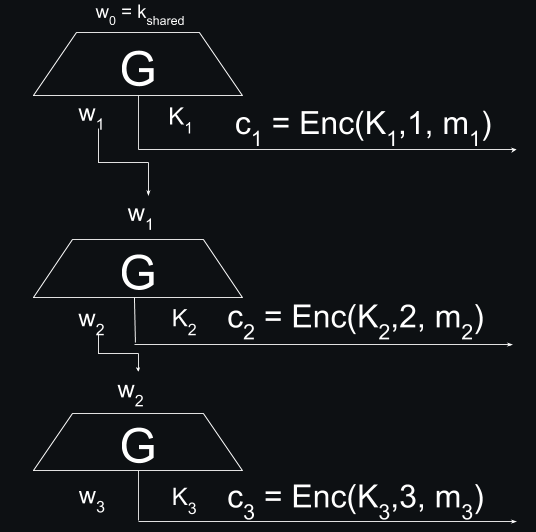
\includegraphics[width=0.95\textwidth]{SendSignal}
%		\end{column}
%		\begin{column}{0.5\textwidth}
%			\centering
%			{\LARGE \color{Orange}\texttt{B}}
%			\pause 
%			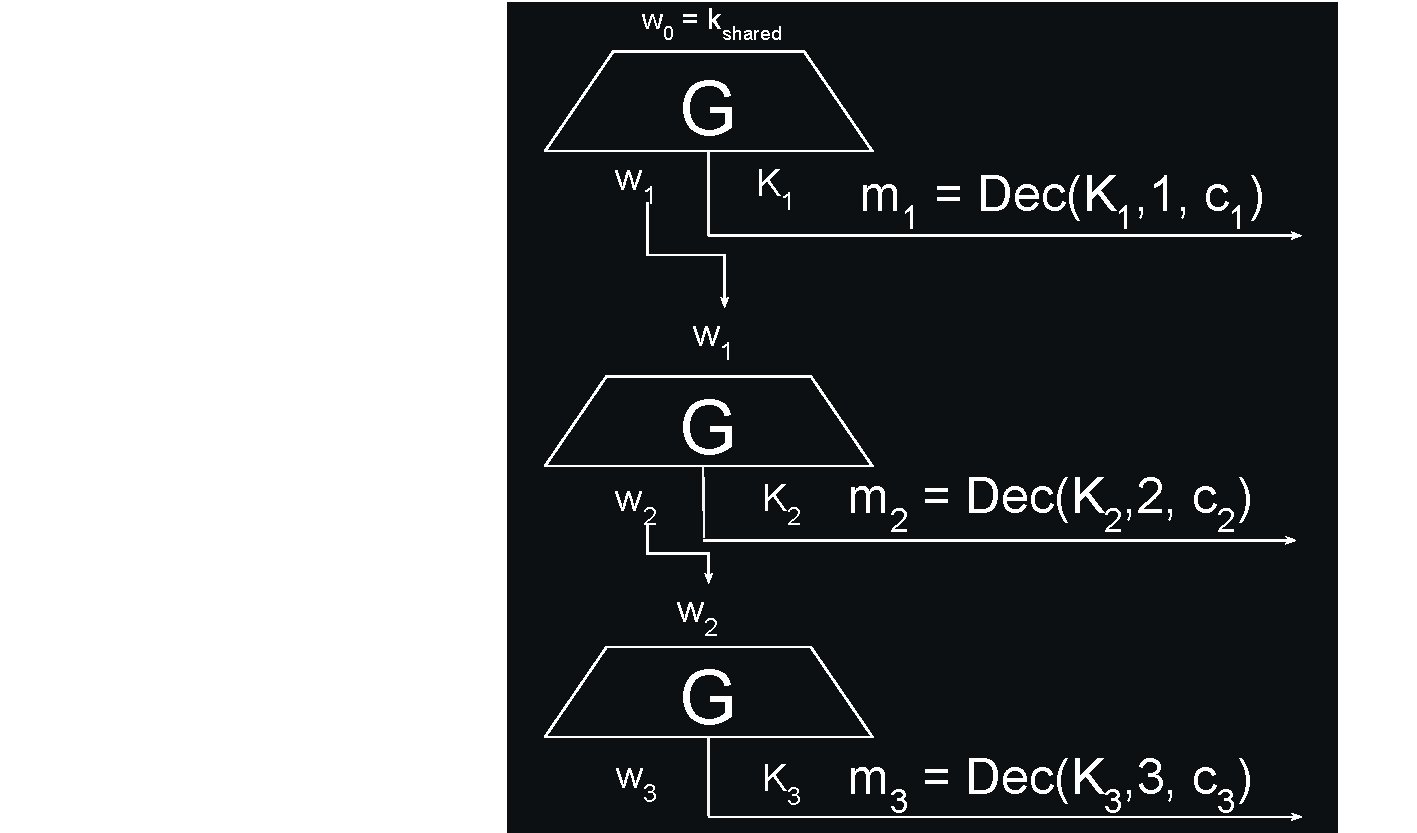
\includegraphics[width=0.95\textwidth]{ReceiveSignal}
%		\end{column}
%	\end{columns}
%\end{frame}
%
%\begin{frame}{Signal: AEAD + PRG}
%Let $\Enc(),\Dec()$ be encryption/decryption procedures of AEAD (see  Lec.\ 7)
%\[
%\text{G}: \{0,1\}^n \rightarrow \{0,1\}^{2n} - \text{cryptographic pseudo-random generator (see Lec. 2)}
%\]
%\vspace{10pt}
%\begin{columns}
%	\begin{column}{0.5\textwidth}
%		\centering
%		{\LARGE \color{Orange}\texttt{A}}
%		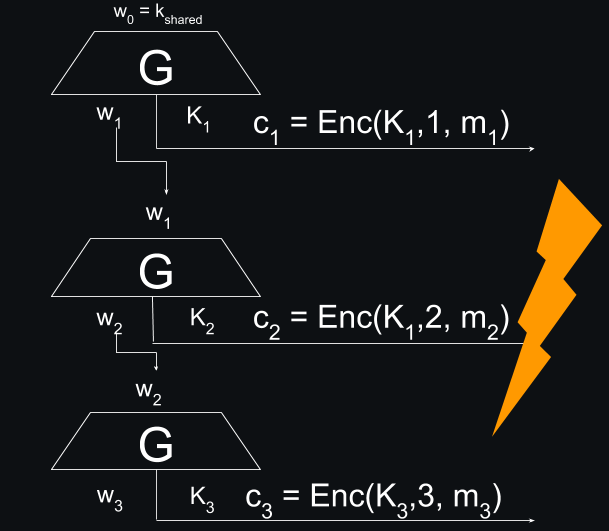
\includegraphics[width=0.95\textwidth]{SendSignalNoC2}
%	\end{column}
%	\begin{column}{0.5\textwidth}
%		\centering
%		{\LARGE \color{Orange}\texttt{B}}
%		\pause 
%		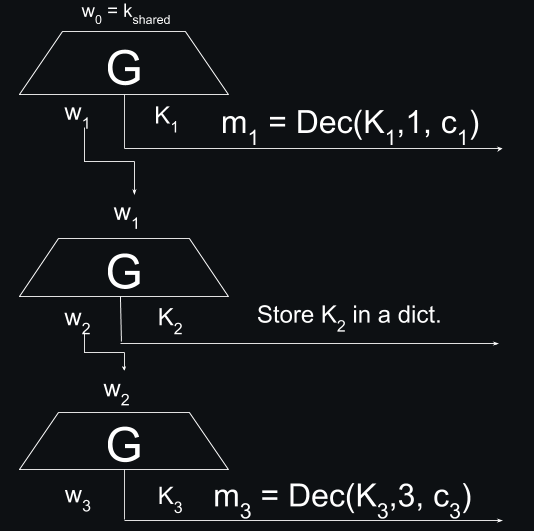
\includegraphics[width=0.95\textwidth]{ReceiveSignalNoC2}
%	\end{column}
%\end{columns}
%\centering
%\vspace{10pt}
%All w$_i$ are erased when no further needed.
%\end{frame}
%
%\begin{frame}{Signal: asymmetric part}
%	\large How to get $k_{\text{shared}} $? \pause You know the answer: use Key Exchange! \\[5pt]
%	Signal is using {\color{Orange} Continuous Key Exchange} based on Diffie-Hellman.
%	\pause 
%	\begin{center}
%		\begin{tabular}{c c c }
%			{\LARGE \color{Orange}\texttt{A}}&    & {\LARGE \color{Orange}\texttt{B}}  \\[5pt]
%			$x_1 $& $\xrightarrow{\hspace{15pt} g^{x_1} \hspace{15pt}}$ & \\
%			& $\xleftarrow{\hspace{15pt} g^{x_2} \hspace{15pt}}$ & $x_2$ \\
%			{\color{Orange}$g^{x_1x_2}$} & & {\color{Orange}$g^{x_1x_2}$} \pause \\[10pt]
%			$x_3 $& $\xrightarrow{\hspace{15pt} g^{x_3} \hspace{15pt}}$ & \\
%			{\color{Orange}$g^{x_2x_3}$} & & {\color{Orange}$g^{x_2x_3}$ }\\[10pt]
%			& $\xleftarrow{\hspace{15pt} g^{x_4} \hspace{15pt}}$ & $x_4$  \\
%			{\color{Orange}$g^{x_3x_4}$} & & {\color{Orange}$g^{x_3x_4}$ }\\
%			& $\vdots $& \\
%		\end{tabular}
%	\end{center}
%
%\normalfont
%\begin{itemize}
%	\item At time $i$ the shared key is $g^{x_i x_{i-1}}$
%	\item A shared key is generated each time a party switches from  {\color{Orange}\texttt{Receiver}} to {\color{Orange}\texttt{Sender}} 
%	\item If at some point $g^{x_i x_{i-1}}$ is compromised (attacker knows $x_i$), the parties recover privacy within two rounds.
%\end{itemize}
%	
%\end{frame}
%
%\begin{frame}{The last slide}
%
%	\centering
%	This is the end of the lectures! \\[10pt]
%	
%	If you want to work on crypto, here is the list of potential projects/thesis topics:
%	
%	\url{https://crypto-kantiana.com/thesis_topics.html}
%	\vfill
%	\pause 
%	Stay healthy and hope to see you soon!
%\end{frame}


\end{document}
